\section{Choix technique}

\par Pour ce projet il a été décidé de réaliser l'architecture serveur/client avec un serveur en java communicant avec le client à l'aide de web socket. L’interface de la messagerie a quant à elle été réalisée à l'aide de technologies web, tout en restant dans le cadre de l'informatique réparti. 

\subsection{Le serveur}
\par Le serveur a entièrement été réalisé en java, et utilise les webSockets de la librairie java-ws pour faire la communication avec le client.
\par L'un des problèmes rencontrés lors du développement du serveur était la persistance des informations, nous avons alors exploré deux options : la sérialisation ou une base de donnée.
Au final notre choix c'est plutôt porté sur la sérialisation parce qu'il s'agissait de la solution la plus simple à implémenter qu'elle convenait mieux pour un petit projet comme celui-ci.
\par Les connexions reçus par le serveur sont traitées avec un système de session, chaque client a une session qui lui est attribuée lors de sa connexion, c'est la session qui permet d'envoyer et de recevoir les requêtes et réponses.
\par Les requêtes prennent forme d'objets JSON avec une action et un contenu. A la réception d'une requête la session fait appelle à un module de décodage qui décode ces requêtes en faisant un Parsing du JSON et appelle la méthode correspondante à l'action grâce à de l'introspection, le reste du contenu de la requête sera mis en paramètre de cette méthode.
\par Chaque requête déclenche l'envoi d'un objet JSON en réponse qui contient à son tour une action, un contenu et un état pour dire si le traitement s'est bien passé.

\subsection{Les web sockets}
\par Les web sockets permettent d'établir la communication entre un client et un serveur. Pour cela nous avons utilisé l'API websocket proposée par HTML pour le client 
et l'API websocket de Java pour le serveur, ce qui nous permet de faire de la communication en temps réel.

\par Les websockets sont une surcouche aux sockets intégrant au dessus un protocole en différentes étapes.
Tout d'abord, au moment de la connexion, le client et le serveur doivent effectuer ce que l'on appelle une poignée de main.
Cette étape permet d'assurer qu'ils sont capables de communiquer sans problème et de définir les modalités d'envoi de message.
Après cette étape, la communication est établit entre le client et le serveur et ils peuvent décider de communiquer l'un avec l'autre 
quand ils le souhaitent sans contrainte de temps, la connexion mise en place étant permanente. 
L'envoi des messages est masqué à l'aide d'un cryptage XOR que le destinataire est capable de décoder.

\section{Guide d'utilisation}

\par Pour lancer l'application il est nécessaire de lancer le serveur puis le client. Pour lancer le serveur il suffit de lancer le compile.sh et le run.sh du dossier serveur et pour lancer le client il faut d'abord installer toutes les dépendances avec npm install puis lancer la commande gulp puis la commande node express.js qui permet d'accéder à la page de connexion sur le navigateur. \\


\par Cette application de messagerie se compose de la manière suivante : \\

\par Au début l'utilisateur accède à une page de login qui lui permet de renseigner son pseudonyme et son mot de passe afin d'accéder au service de messagerie. Si l'utilisateur est nouveau, il a la possibilité de créer son compte en renseignant son pseudonyme, adresse mél, mot de passe, nom, prénom et date de naissance. 
\par Une fois l'authentification faite l'utilisateur accède à la page principale qui correspond à la page d'historique des conversations des utilisateurs. L'utilisateur peut ainsi sélectionner une conversation déjà existante ou bien en créer une nouvelle. Il a la possibilité de choisir parmi les membres du service messagerie la personne qu'il veut joindre. Il accède ensuite à la page de cette nouvelle conversation. Il peut discuter avec les personnes membres de la messagerie ou bien avec l'IA : MiaBot.
\par Via la navbar il est possible d'accéder au carnet d'adresse et à la page de paramètres. \\

Voici les captures d'écran de l'application que nous avons réalisée.



\begin{figure}[H]
   \begin{minipage}[c]{.46\linewidth}
      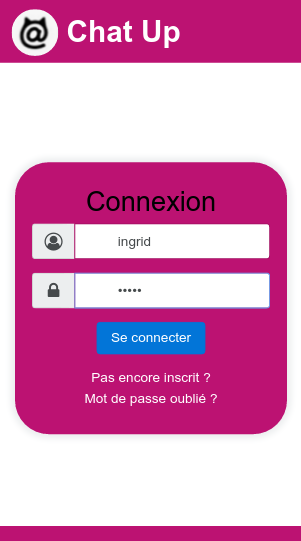
\includegraphics[scale=0.5]{img/01Login.png}
      \caption{Page de connexion}
   \end{minipage} \hfill
   \begin{minipage}[c]{.46\linewidth}
      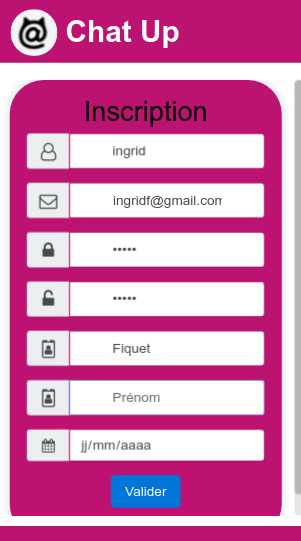
\includegraphics[scale=0.5]{img/02InscriptionChamp.png}
      \caption{Page d'inscription}
   \end{minipage}
\end{figure}


\begin{figure}[H]
   \begin{minipage}[c]{.46\linewidth}
		\centering 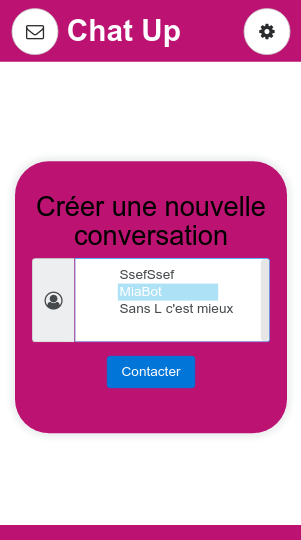
\includegraphics[scale=0.5]{img/03ChoixMsg.png}
		\caption{Page de Création d'une conversation}
   \end{minipage} \hfill
   \begin{minipage}[c]{.46\linewidth}
		\centering 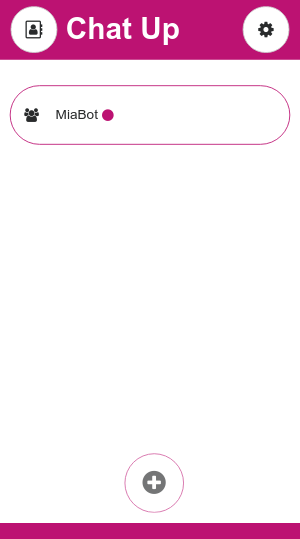
\includegraphics[scale=0.5]{img/05HistoriqueMessagerie.png}
		\caption{Page de Messagerie}
   \end{minipage}
\end{figure}

\begin{figure}[H]
   \begin{minipage}[c]{.46\linewidth}
		\centering 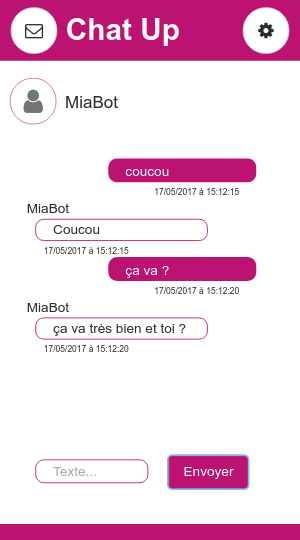
\includegraphics[scale=0.5]{img/04Messagerie.png}
		\caption{Conversation textuelle}
   \end{minipage} \hfill
   \begin{minipage}[c]{.46\linewidth}
		\centering 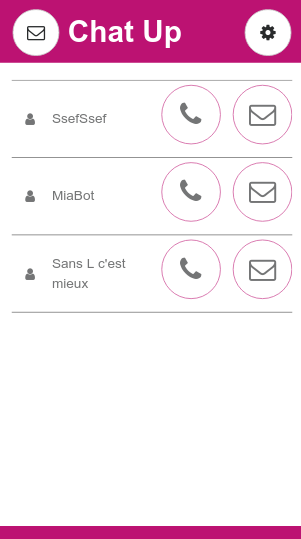
\includegraphics[scale=0.5]{img/06ContactMessagerie.png}
		\caption{Page de contacts}
   \end{minipage}
\end{figure}


\begin{figure}[H]
   \begin{minipage}[c]{.46\linewidth}
		\centering 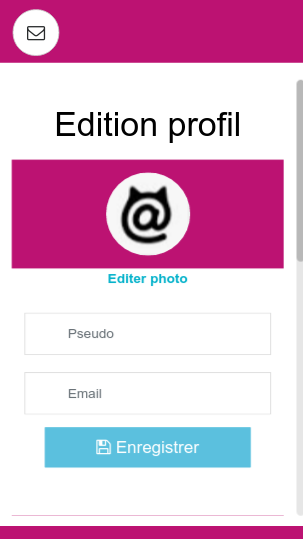
\includegraphics[scale=0.5]{img/07Param.png}
		\caption{Page de paramètres}
   \end{minipage} \hfill
   \begin{minipage}[c]{.46\linewidth}
		\centering 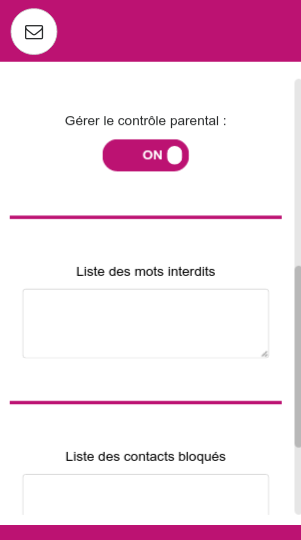
\includegraphics[scale=0.5]{img/08paramsuite.png}
		\caption{Page de paramètres}
   \end{minipage}
\end{figure}

 


\section{Tests de validation}

Voici la liste des tests de validation qui ont été réalisés. \\

%TODO mettre que les tests qui ont été réalisé 

\paragraph{Spécifications fonctionnelles\\} 

Voici la liste des tests qui ont été réalisés techniquement :
\begin{itemize}
	\item Créer un nouveau compte ;
	\item Obtenir la liste des conversations ;
	\item Créer une conversation ;
	\item Faire une conversation avec plusieurs utilisateurs dans une conversation textuelle ; 
	\item Créer des filtres (du côté serveur);
\end{itemize}

Les tests suivant ont été réalisés de manière manuelle : 
\begin{itemize}
	\item Se connecter et se déconnecter ;
	\item Voir la liste des autres utilisateurs ;
	\item Envoyer un message dans une conversation ;
	\item Recevoir un message dans une conversation ;
	\item Voir l'historique d'une conversation après reprise ;
	\item Activer et désactiver le contrôle parental ;
	\item Créer des filtres (du côté client);
	\item Filtrer des messages ; 
	\item Avoir une conversation minimaliste avec l'IA ; \\
\end{itemize}

\paragraph{Spécifications d'interface \\}

En ce qui concerne les spécifications d'interface, nous avons bien réalisé une application responsive design, consultable sur un écran de taille d'ordinateur, de tablette ou de smartphone. De plus, l'application est intuitive et facile d'utilisation.

\paragraph{Spécifications opérationnelles \\}

Nous avons répondu aux spécifications opérationnelles suivantes :
\begin{itemize}
	\item Rapidité de la discussion instantanée ; 
	\item Discussions privées et uniquement visibles par les membres de la conversation ;
	\item Mot de passe hashé. \\
\end{itemize}